%%%%%%%%%%%%%%%%%%%%%%%%%
%% Header for standard beamer presentation
%%
%%  PresentationHeader.tex
%%
%%%%%%%%%%%%%%%%%%%%%%%%%

\documentclass[english,10pt]{beamer}

%%%%%%%%%%%%%%%%%%%%
%% Include general header where common packages are defined
%%%%%%%%%%%%%%%%%%%%

% general packages without options
\usepackage{amsmath,amssymb,bbm}




%%%%%%%%%%%%%%%%%%%%
%% Idem general commands
%%%%%%%%%%%%%%%%%%%%

%%% Commands

\newcommand{\noun}[1]{\textsc{#1}}


%% Math

% Operators
\DeclareMathOperator{\Cov}{Cov}
\DeclareMathOperator{\Var}{Var}
\DeclareMathOperator{\E}{\mathbb{E}}
\DeclareMathOperator{\Proba}{\mathbb{P}}

\newcommand{\Covb}[2]{\ensuremath{\Cov\!\left[#1,#2\right]}}
\newcommand{\Eb}[1]{\ensuremath{\E\!\left[#1\right]}}
\newcommand{\Pb}[1]{\ensuremath{\Proba\!\left[#1\right]}}
\newcommand{\Varb}[1]{\ensuremath{\Var\!\left[#1\right]}}

% norm
\newcommand{\norm}[1]{\| #1 \|}


% amsthm environments
\newtheorem{definition}{Definition}



%% graphics

% renew graphics command for relative path providment only ?
%\renewcommand{\includegraphics[]{}}






\usetheme{Warsaw}

\setbeamertemplate{footline}[text line]{}
\setbeamercolor{structure}{fg=purple!50!blue, bg=purple!50!blue}

\setbeamercovered{transparent}


% shortened command for a justified frame
\newcommand{\jframe}[2]{\frame{\frametitle{#1}\justify{#2}}}



%%%%%%%%%%%%%%%%%%%%%
%% Begin doc
%%%%%%%%%%%%%%%%%%%%%

\begin{document}


\title{Thesis Progress Meeting}


\author{J.~Raimbault$^{1,2}$}

\institute{$^{1}$G{\'e}ographie-Cit{\'e}s (UMR 8504 CNRS)\\
$^{2}$LVMT (UMR-T 9403 IFSTTAR)}


\date{April 17th 2015
}


%%%%%%%%%%%%%%%%%%%%%%%%%%%%%%%%
\begin{frame}
\titlepage
\end{frame}

\begin{frame}
\tableofcontents
\end{frame}
%%%%%%%%%%%%%%%%%%%%%%%%%%%%%%%%


\section{Current Projects}

\jframe{Current Projects}{
\begin{enumerate}
\item General Bibliography - Subject and Question precision.
\item Technical Tools : development of tools, getting started with others.
\item Algorithmic Systematic Review
\item Existing Model Quantitative Benchmarking
\item Theoretical Model Coupling
\item Control of meta-parameters through synthetic data
\item Governance
\item Scaling Sensitivity
\end{enumerate}
}



\section{Achieved Work}


\jframe{Achieved Work (by projects)}{
\begin{itemize}
\item Technical Tools
\begin{itemize}
\item OpenMole Workflow with NetLogo tasks, running on remote. [1w]
\item NetLogoDoc, tool to automatically generate elaborated documentation from NL code. [0.5w]
\end{itemize}
\item General Bibliography. [0.3w]
\item Algorithmic Systematic Review
\begin{itemize}
\item Google Scholar API to check catalog validity and retrieve citing refs. [0.5w]
\item Short Paper for ECTQG. [0.3w]
\end{itemize}
\item Synthetic Data Control : simple macro-model, calibrated through mrophological indicators on european density data. [0.5w]
\item Governance : theoretical game-theory model, old implementation recoding. [0.5w]
\item Scaling Sensitivity : theoretical derivation of phase diagram. [0.3w]
\end{itemize}
}



\section{Technical Developments}


\jframe{NetLogoDoc}{
$\rightarrow$ Need for a systematic documentation of model, including internal implementation (generally not systematically vlidated).
\bigskip
Filter transforming NL code into intermediary java code, processed by \texttt{Doxygen}. Helps for architecture as analogy with classes has to be found (\texttt{.nls} correspond mainly to static classes in our convention).

\bigskip
TODO : release beta version for testing.

}

\jframe{Algo SR}{
Scholar API allows to retrieve citing references (only this sense).
\bigskip

$\rightarrow$ External validation of classification results for corpuses obtained through langage processing through study of clustering coefficients for 1st order backward citation network.

\bigskip

TODO : compute clustering coefs, finish paper ECTQG.

}


\jframe{Synthetic Data Control}{

Gibrat model, valid in first approximation~\cite{favaro2011gibrat}, used to generate macro-distribution of densities - strongly coupled with an heterogeneous diffusion model to obtain spatially distributed ``cities''.

\bigskip

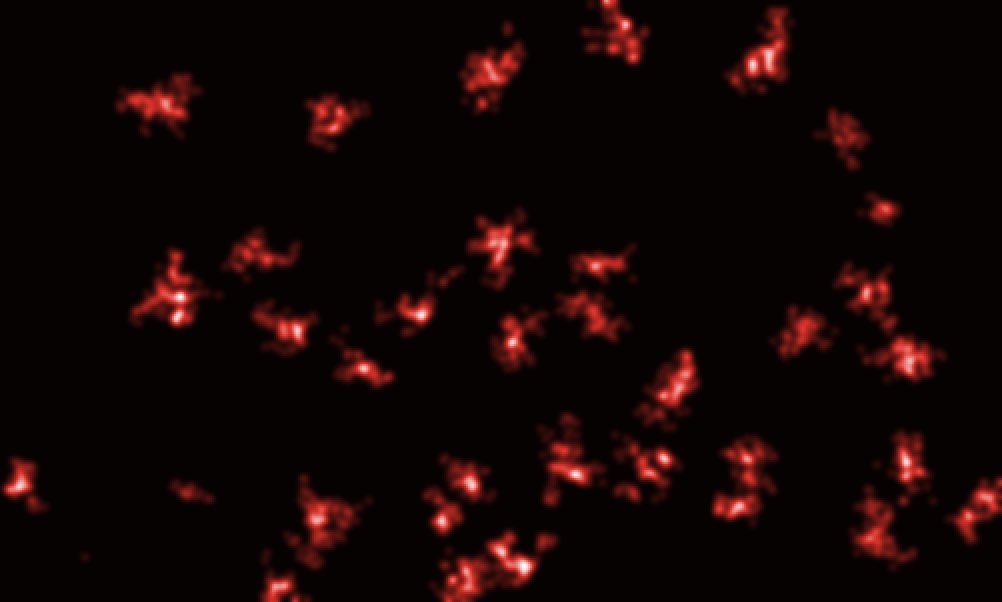
\includegraphics[width=0.45\textwidth]{figures/gibrat1}\hfill
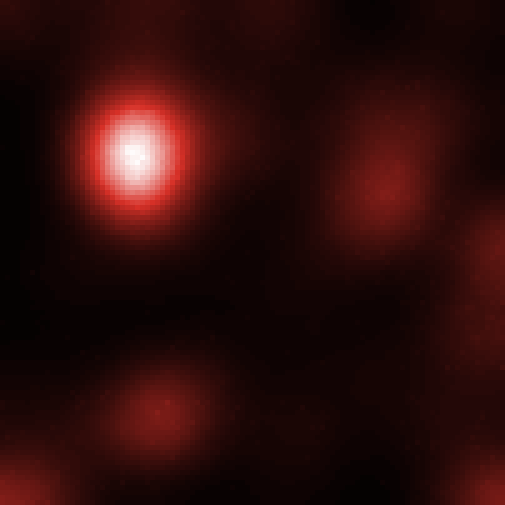
\includegraphics[width=0.45\textwidth,height=0.35\textheight]{figures/gibrat2}
    
}

\jframe{Synthetic Data Control}{
Currently being calibrated on real data (Greater Paris and London).

\bigskip

Identification of plausible parameter values, associated to different thematic regimes~\cite{duranton1999distance}

\bigskip

$\rightarrow$ Generation of stochastic datasets of synthetic macro-distribution for densities, on which one can control e.g. the transition from ``tyranny of distance'' to ``tyranny of land''. Use of these controls to study behavior of morphogenesis models that take macro density profiles as exogeneous variables.
}


\jframe{Governance}{

Original model in~\cite{lenechet2012} : LUTI model with the originality to have an evolving transportation network infrastructure, depending on a gouvernance structure.

\bigskip

Extension : test the effects of possible evolution of gouvernance structure (e.g. merge of communes). Can a polycentric metropolis emerge from the bottom-up ?

\bigskip

$\rightarrow$ Game-theory framework to express negociations between adjacent cities when building new infrastructures ; local rules for constructing and/or merging.

\bigskip

TODO : finish a functional implementation (to slow for now).

\textit{Abstract for ECTQG}

}


\jframe{Scaling}{

Based on~\cite{2013arXiv1301.1674A}, current work by C. Cottineau : phase diagrams of scaling parameter for different urban variables in the 2D space of morphological and functional threshold used to define boundaries of cities.

\bigskip

\textbf{Q : } Form of the phase diagram should contain structure of the urban system ? In particular relationship between form and function ?

\bigskip

\textbf{Current Work : } Formal derivation of the expression of the phase diagram for Gaussian Mixtures, to check if results are not structural.

\bigskip

TODO : Should be interesting to look at variation of phase diagram across varying geographical ragions (position and size), may confirm different mechanisms of systems of cities.

}



%%%%%%%%%%%%%%%%%%%%%%%%%%%%%%%%
\begin{frame}[allowframebreaks]
\frametitle{References}
\bibliographystyle{apalike}
\bibliography{/Users/Juste/Documents/ComplexSystems/CityNetwork/Biblio/Bibtex/CityNetwork}
\end{frame}
%%%%%%%%%%%%%%%%%%%%%%%%%%%%%%%%


\end{document}